\chapter[Continuous distributions]{Continuous variables: Population and sampling distributions}
\label{c_contd}

\section{Introduction}
\label{s_contd_intro}

This chapter serves both as an explanation of some topics that
were skimmed over previously, and as preparation for later
chapters. Its central theme is probability distributions
of continuous variables. These may appear
in two distinct roles:
\begin{itemize}
\item
As population distributions of continuous variables, for instance blood
pressure in the illustrative example of this chapter. This contrasts with
the kinds of discrete variables that were considered in Chapters
\ref{c_tables} and \ref{c_probs}. Methods of inference for continuous
variables will be introduced in Chapters \ref{c_means} and
\ref{c_regression}.
\item
As sampling distributions of sample statistics. These are
typically continuous even in analyses of discrete variables, such as in
Chapter \ref{c_probs} where the variable of interest $Y$ was binary but
the sampling distributions of a sample proportion $\hat{\pi}$ and
the $z$-test statistic for population probability $\pi$ were
nevertheless continuous. We have already encountered two continuous
distributions in this role, the $\chi^{2}$ distributions in Chapter
\ref{c_tables} and the standard normal distribution in Chapter
\ref{c_probs}. Their origins are explained in more detail below.
\end{itemize}


\label{p_bpressure_ex}
%\textbf{\underline{Example 6.1}: Survey data on blood pressures}

To illustrate the concepts, we use data from the Health Survey for
England 2002 (HES).\footnote{Carried out on behalf of The Department of
Health by SCPR and the Department of Epidemiology and Public Health,
UCL. Data used here were obtained from the UK Data Archive at
\texttt{www.data-archive.ac.uk}.} One part of the survey was a short
physical examination by a nurse. Figure \ref{f_bp1} shows a histogram
and frequency polygon of diastolic blood pressure (in mm Hg) for 4489
respondents, measured by the mean of the last two of three measurements
taken during the examination. Data from respondents for whom the
measurements were not obtained or were considered invalid have been
excluded. Respondents aged under 25 have also been excluded for
simplicity, because this age group was oversampled in the 2002 HES.

\begin{figure}
\caption{Histogram of diastolic blood pressure, with the corresponding
frequency polygon, from Health Survey for
England 2002 (respondents aged 25 or over, $n=4489$).}
\label{f_bp1}
\begin{center}
\vspace*{-4ex}
%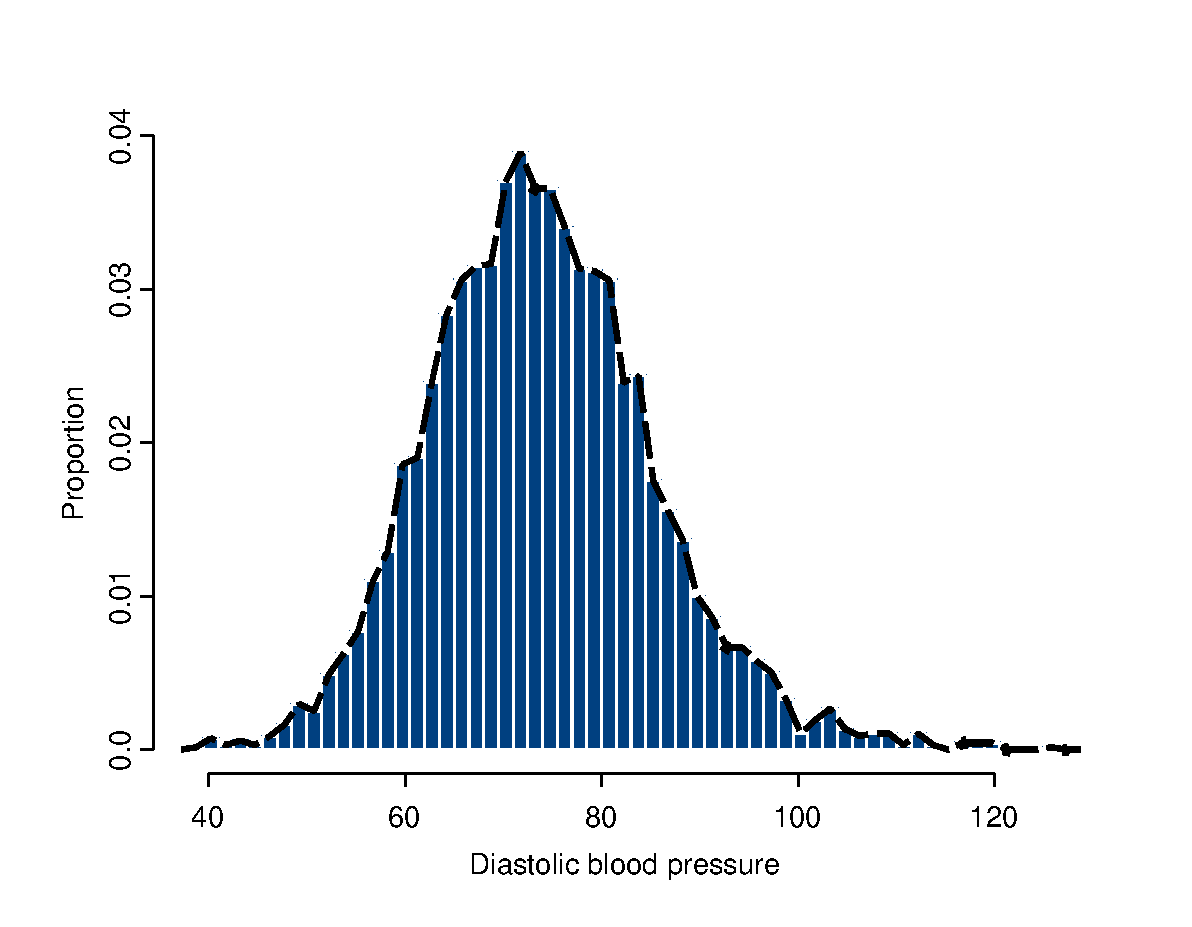
\includegraphics[height=9cm]{bloodp1}
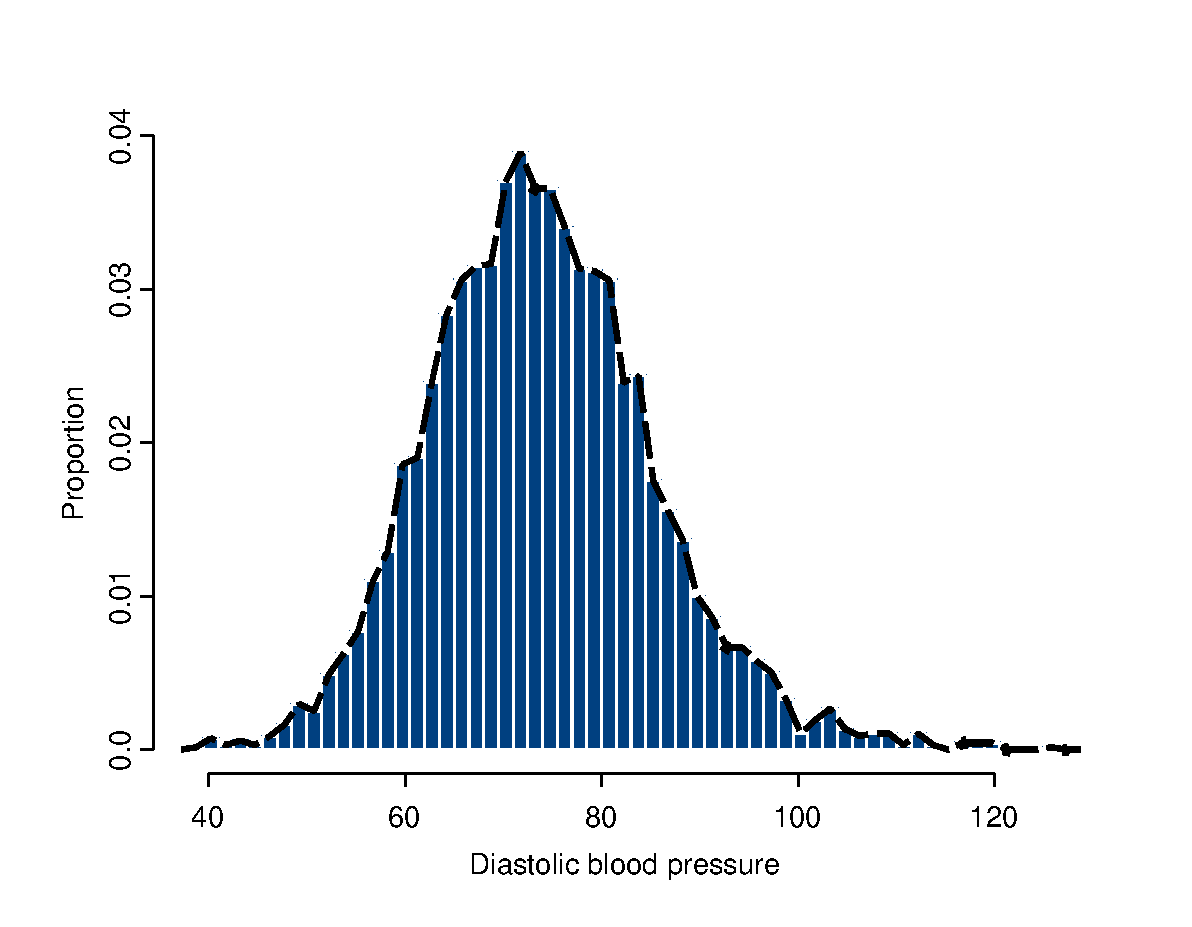
\includegraphics[width=13.5cm]{bloodp1}
\end{center}
%\vspace*{-4ex}
\end{figure}

The respondents whose blood pressures are summarized in Figure
\ref{f_bp1} are in reality a sample from a larger population in the
sense of Sections \ref{s_samples_finpops} and \ref{s_samples_samples}.
However, for illustrative purposes we will here pretend that they are
actually an entire finite population of 4489 people (the adults in a
small town, say). The values summarised in Figure \ref{f_bp1} then form
the population distribution of blood pressure in this population. It is
clear that blood pressure is best treated as a continuous variable.


\section{Population distributions of continuous variables}
\label{s_contd_popdistrs}

\subsection{Population parameters and their point estimates}
\label{ss_contd_popdistrs_params}

If we knew all of its values, we could summarise a finite population
distribution by, say, a histogram like Figure \ref{f_bp1}. We
can also consider specific characteristics of the distribution, i.e.\
its \emph{parameters} in the sense introduced in Section
\ref{s_probs_distribution}. For the distribution of a  continuous variable, the most
important parameters are the \textbf{population mean}
\begin{equation}
\mu=\frac{\sum Y_{i}}{N}
\label{mu}
\end{equation}
and the \textbf{population variance}
\begin{equation}
\sigma^{2} = \frac{\sum (Y_{i}-\mu)^{2}}{N}
\label{sigma2}
\end{equation}
or, instead of the variance, the \textbf{population standard deviation}
\begin{equation}
\sigma = \sqrt{\frac{\sum (Y_{i}-\mu)^{2}}{N}}.
\label{sigma}
\end{equation}
Here $\mu$ and $\sigma$ are the lower-case Greek letters ``mu'' and
``sigma'' respectively, and $\sigma^{2}$ is read ``sigma squared''. It
is common to use Greek letters for population parameters, as we did also
for the probability parameter $\pi$ in Chapter \ref{c_probs}.

In (\ref{mu})--(\ref{sigma}), $N$ is the number of units in a finite
population and the sums indicated by $\Sigma$ are over all of
these $N$ units. If we treat the data in Figure \ref{f_bp1} as a
population, $N=4489$ and these population parameters are $\mu=74.2$,
$\sigma^{2}=127.87$ and $\sigma=11.3$.

Because the formulas (\ref{mu})--(\ref{sigma}) involve the population
size $N$, they apply in this exact form only to finite populations like
the one in this example (and as discussed more generally in Section
\ref{s_samples_finpops}) but not to infinite ones of the kind discussed
in Section \ref{s_samples_infpops}. However, the definitions of $\mu$,
$\sigma^{2}$, $\sigma$ and other parameters can be extended to apply
also to infinite populations. These definitions, which will be omitted
here, involve the concept of continuous probability distributions that
is discussed in the next section. The interpretations of the population
parameters turn out to be intuitively similar for both the finite and
infinite-population cases, and the same methods of analysis apply to
both, so we can here ignore the distinction without further comment.

The population formulas (\ref{mu})--(\ref{sigma}) clearly resemble those of
some sample statistics introduced in Chapter
\ref{c_descr1}, specifically the \emph{sample} mean, variance and
standard deviation
\begin{eqnarray}
\bar{Y}&=&\frac{\sum Y_{i}}{n}, \label{Ybar_ch6} \\[.3ex]
s^{2} &=& \frac{\sum (Y_{i}-\bar{Y})^{2}}{n-1} \hspace*{1em}\text{and}
\label{s2_ch6} \\[.3ex]
s &=& \sqrt{\frac{\sum (Y_{i}-\bar{Y})^{2}}{n-1}}
\label{s_ch6}
\end{eqnarray}
where the sums are now over the $n$ observations in a sample. These can
be used as descriptions of the sample distribution as discussed in
Chapter \ref{c_descr1}, but also as \emph{point estimates} of the
corresponding population parameters in the sense defined in Section
\ref{s_probs_pointest}. We may thus use the sample mean $\bar{Y}$ as a
point estimate of the population mean $\mu$, and the sample variance
$s^{2}$ and sample standard deviation $s$ as point estimates of
population variance $\sigma^{2}$ and standard deviation $\sigma$
respectively. These same estimates can be used for both finite and
infinite population distributions.

For further illustration of the connection between population and
sample quantities, we have also drawn a simple random sample of $n=50$
observations from the finite population of $N=4489$ observations in
Figure \ref{f_bp1}. Table \ref{t_bp_example} shows the summary
statistics (\ref{Ybar_ch6})--(\ref{s_ch6}) in this sample and the
corresponding parameters (\ref{mu})--(\ref{sigma}) in the population.

\begin{table}
\caption{Summary statistics for diastolic blood pressure in the
population and a sample from it in the example used for illustration
in Sections \ref{s_contd_popdistrs}--\ref{s_contd_clt}.}
\label{t_bp_example}
\begin{center}
\begin{tabular}{|l|rrrr|}\hline
& & & Standard & \\
& Size & Mean & Deviation & Variance \\ \hline
Population
\rule[-3mm]{0mm}{8mm}
& $N=4489$ & $\mu=74.2$ & $\sigma=11.3$ &
$\sigma^{2}=127.87$ \\ \hline
Sample
\rule[-3mm]{0mm}{8mm}
& $n=50$ & $\bar{Y}=72.6$ & $s=12.7$ & $s^{2}=161.19$ \\
\hline
\end{tabular}
\end{center}
\end{table}

You may have noticed that the formulas of the sample variance
(\ref{s2_ch6}) and sample standard deviation (\ref{s_ch6}) involve the
divisor $n-1$ rather than the $n$ which might seem more natural, while
the population formulas (\ref{sigma2}) and (\ref{sigma}) do use $N$
rather than $N-1$. The reason for this is that using $n-1$ gives the
estimators certain mathematically desirable properties ($s^{2}$ is an \emph{unbiased} estimate of $\sigma^{2}$, but
$\hat{\sigma}^{2}$ below is not). This detail need not concern us here.
In fact, the statistics which use $n$ instead, i.e.\
\begin{equation}
\hat{\sigma}^{2}=\frac{\sum (Y_{i}-\bar{Y})^{2}}{n}
\label{s2b}
\end{equation}
for $\sigma^{2}$ and $\hat{\sigma}=\sqrt{\hat{\sigma}^{2}}$ for
$\sigma$, are also sensible estimates and very similar to
$s^{2}$ and $s$ unless $n$ is very small. In general, there are often
several possible sample statistics which could be used as estimates for
the same population parameter.

\section{Probability distributions of continuous variables}
\label{s_contd_probdistrs}

\subsection{General comments}
\label{ss_contd_probdistrs_general}

Thinking about population distributions of continuous distributions
using, say, histograms as in Figure \ref{f_bp1} would present
difficulties for statistical inference, for at least two reasons. First,
samples cannot in practice give us enough information to make reliable
inferences on all the details of a population distribution, such as the
small kinks and bumps of Figure \ref{f_bp1}. Such details would
typically not even be particularly interesting compared to major
features like the central tendency and variation of the population
distribution. Second, this way of thinking about the population
distribution is not appropriate when the population is regarded as
infinite.

Addressing both of these problems requires one more conceptual leap.
This is to make the assumption that the population distribution is
well-represented by a continuous \emph{probability distribution}, and
focus on inference on the parameters of that distribution.

We have already introduced the concept of probability distributions in
Section \ref{s_samples_popdistrs},  and considered instances of it in
Chapters \ref{c_tables} and \ref{c_probs}. There, however, the term was
not emphasised because it added no crucial insight into the
methods of inference. This was because for discrete variables a
probability distribution is specified simply by listing the
probabilities of all the categories of the variable. The additional
terminology of probability distributions and their parameters seems
almost redundant in that context.

The situation is very different for continuous variables. This is
illustrated by Figure \ref{f_bp2}, which shows the same frequency
polygon as in Figure \ref{f_bp1}, now supplemented by a
smooth curve. This curve (``a probability density
function'') describes a particular probability distribution. It can be
thought of as a smoothed version of the shape of the frequency polygon.
What we will do in the future is to use some such probability
distribution to represent the population distribution. This means
effectively arguing that we believe that the shape of the true
population distribution is sufficiently regular to be well described by
a smooth curve such as the one in Figure \ref{f_bp2}.

In Figure \ref{f_bp2} the curve and the frequency polygon have
reasonably similar shapes, so the assumption that the former is a
good representation of the latter does not seem far-fetched. However, the two are
clearly not exactly the same, \label{p_model2} nor do we expect that
even the blood pressures of all English adults exactly match
this curve or any other
simple probability distribution. All we require is that a
population distribution is close enough to a specified probability
distribution for the results from analyses based on this assumption to
be meaningful and not misleading.


\begin{figure}
\caption{The frequency polygon of Figure \ref{f_bp1},
together with a normal curve with the same mean and variance.}
\label{f_bp2}
\begin{center}
\vspace*{-4ex}
%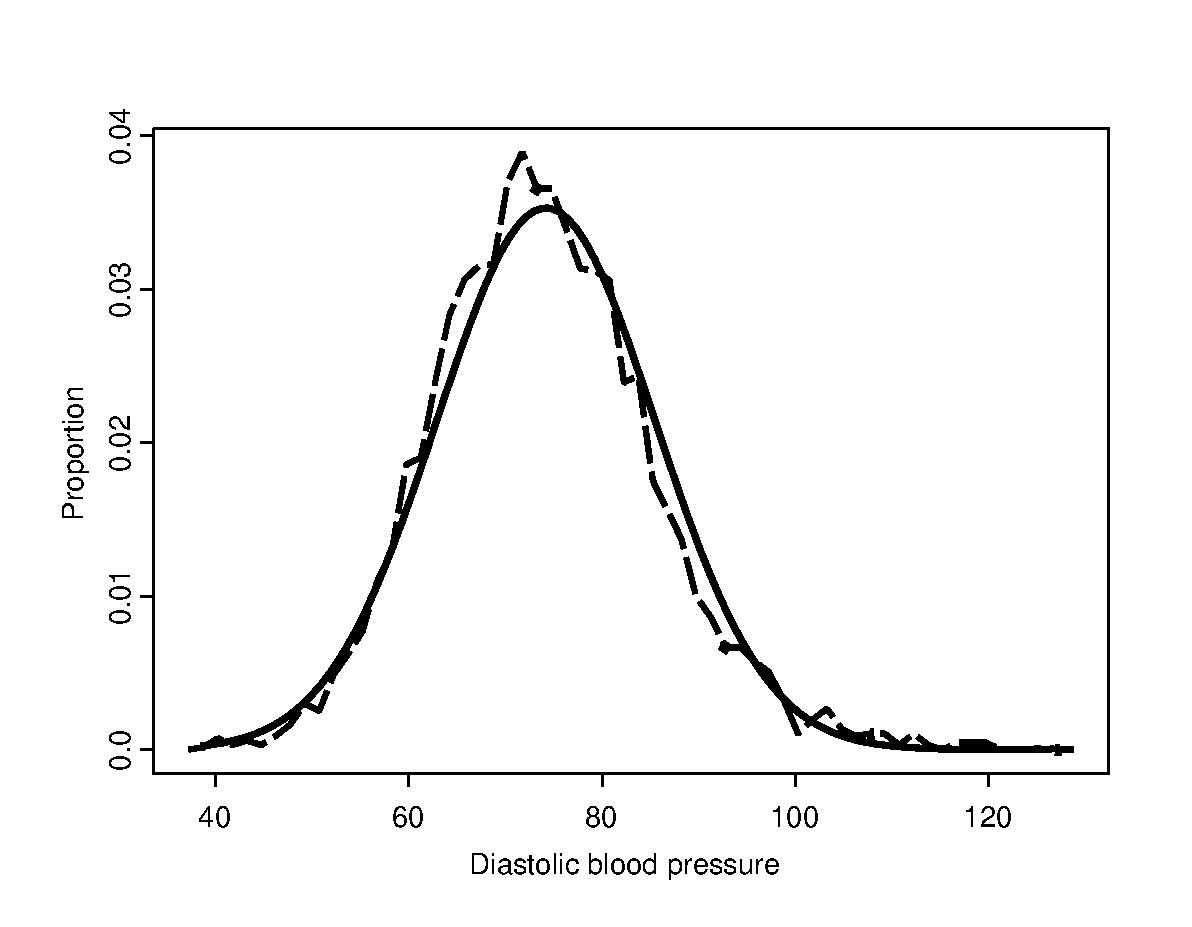
\includegraphics[height=8.5cm]{bloodp2}
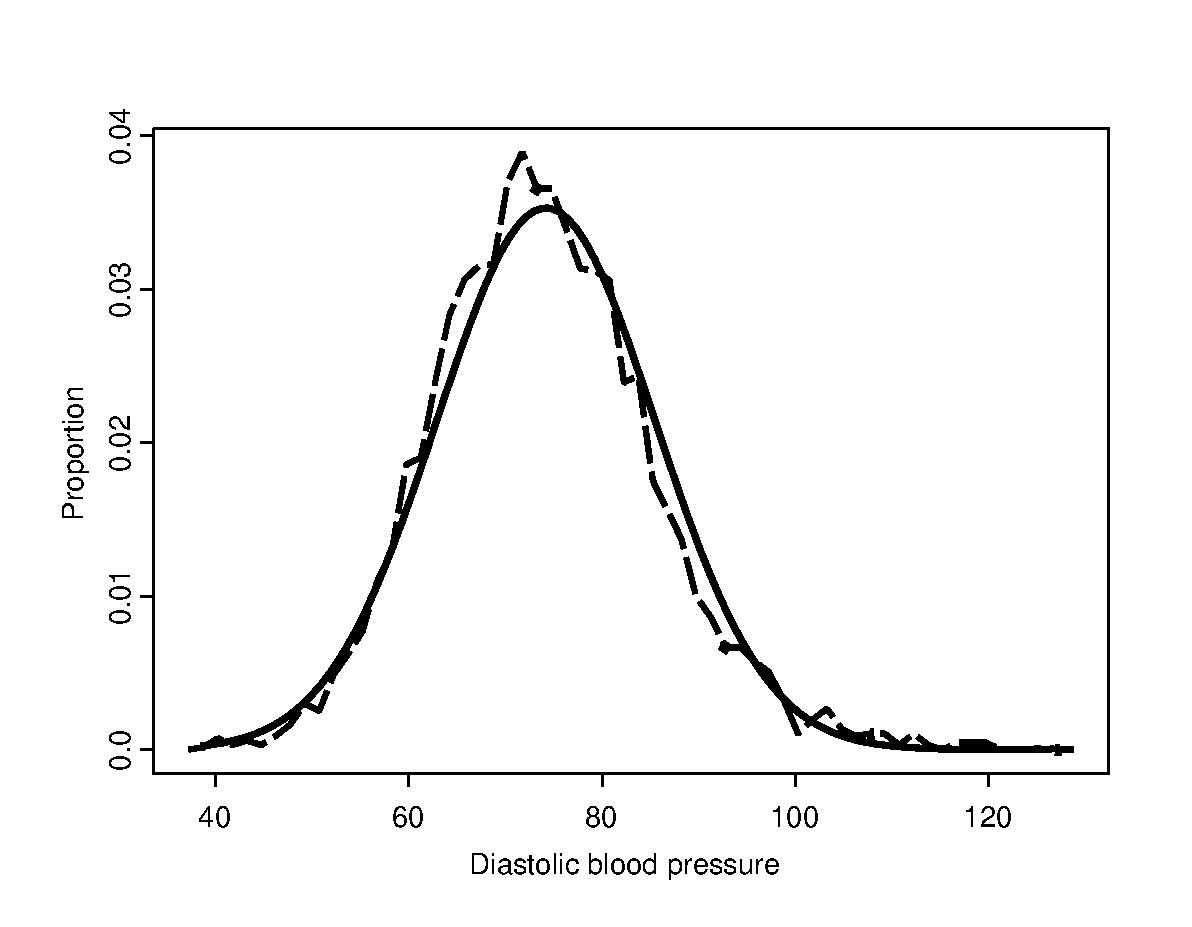
\includegraphics[width=11.5cm]{bloodp2}
\end{center}
\vspace*{-3ex}
\end{figure}

\label{p_model}
Such a simplifying assumption about
the population distribution is known as a \textbf{statistical model} for
the population.
The reason for working with a model is that it leads to much
simpler methods of analysis than would otherwise be required. For
example, the shape of the distribution shown in Figure \ref{f_bp2} is
entirely determined by just two parameters, its mean and variance.
Under this model, all questions about the population distribution
can thus be reduced to questions about these two
population parameters, and inference can focus on tests and confidence
intervals for them.

The potential cost of choosing a specific probability distribution as
the statistical model for a particular application is that the
assumption may be inappropriate for the data at hand, and if it is,
conclusions about population parameters derived from analyses based on
this assumption may be misleading. The distribution should thus be
chosen carefully, usually based on both substantive considerations and
initial descriptive examination of the observed data.

For example, the particular probability distribution shown in Figure
\ref{f_bp2}, which is known as the normal distribution, is by definition
symmetric around its mean. While it is an adequate approximation of many
approximately symmetric population distributions of continuous
variables, such as that of blood pressure, many other population
distributions are not even roughly symmetric. It would be unrealistic to
assume the population distributions of such variables to be normal.
Instead, we might consider other continuous probability distributions
which can be skewed. Examples of these are the \emph{Exponential},
\emph{Gamma}, \emph{Weibull}, and \emph{Beta} distributions.
\emph{Discrete} distributions, of course, will require quite different
probability disributions, such as the \emph{Binomial} distribution
discussed in Chapter \ref{c_probs}, or the \emph{Multinomial} and
\emph{Poisson} distributions. On this course, however, we will not
include further discussion of these various possibilities.

\subsection{The normal distribution as a population distribution}
\label{ss_contd_probdistrs_normal}

The particular probability distribution that is included in Figure
\ref{f_bp2} is a \textbf{normal distribution}, also known as the
\emph{Gaussian} distribution, after the great German mathematician Karl
Friedrich Gauss who was one of the first to derive it in 1809. Figure
\ref{f_10dm} shows a portrait of Gauss from the former German 10-DM
banknote, together with pictures of the university town of G\"{o}ttingen
and of the normal curve (even the mathematical formula of the curve is
engraved on the note). The curve of the normal distribution is also
known as the ``bell curve'' because of its shape.

\begin{figure}
\caption{A portrait of Gauss and the normal curve on a former German
10-DM banknote.}
\label{f_10dm}

\includegraphics[width=14cm]{mark}
\end{figure}

The normal distribution is by far the most important probability
distribution in statistics. The main reason for this is its use as a
sampling distribution in a wide range of contexts, for reasons that are
explained in Section \ref{s_contd_clt}. However, the normal distribution
is also useful for describing many approximately symmetric population
distributions, and it is in this context that we introduce its
properties first.

A normal distribution is completely specified by two
numbers, its mean (or ``expected value'') $\mu$ and variance $\sigma^{2}$. This is
sometimes expressed in notation as $Y\sim N(\mu, \sigma^{2})$, which is read
as ``$Y$ is normally distributed with mean $\mu$ and variance
$\sigma^{2}$''. Different values for $\mu$ and $\sigma^{2}$ give
different distributions. For example, the curve in Figure \ref{f_bp2} is
that of the $N(74.2, \, 127.87)$ distribution, where the mean $\mu=74.2$
and variance $\sigma^{2}=127.87$ are the same as the mean
and variance calculated from formulas (\ref{mu}) and (\ref{sigma2}) for
the 4489 observations of blood pressure. This ensures that this
particular normal curve best matches the frequency polygon in Figure \ref{f_bp2}.

The mean $\mu$ describes the central tendency of the
distribution, and the variance $\sigma^{2}$ its variability. This is
illustrated by Figure \ref{f_3norms}, which shows the curves for three
different normal distributions. The mean of a normal distribution is
also equal to both its median and its mode. Thus $\mu$ is the central
value in the sense that it divides the distribution into two equal
halves, and it also indicates the peak of the curve (the highest
probability, as discussed below). In Figure \ref{f_3norms}, the curves
for $N(0, 1)$ and $N(0, 9)$ are both centered around $\mu=0$; the mean
of the $N(5, 1)$ distribution is $\mu=5$, so the whole curve is shifted
to the right and centered around 5.

\begin{figure}
\caption{Three normal distributions with different means and/or
variances.}
\label{f_3norms}
%\vspace*{-2ex}
\begin{center}
%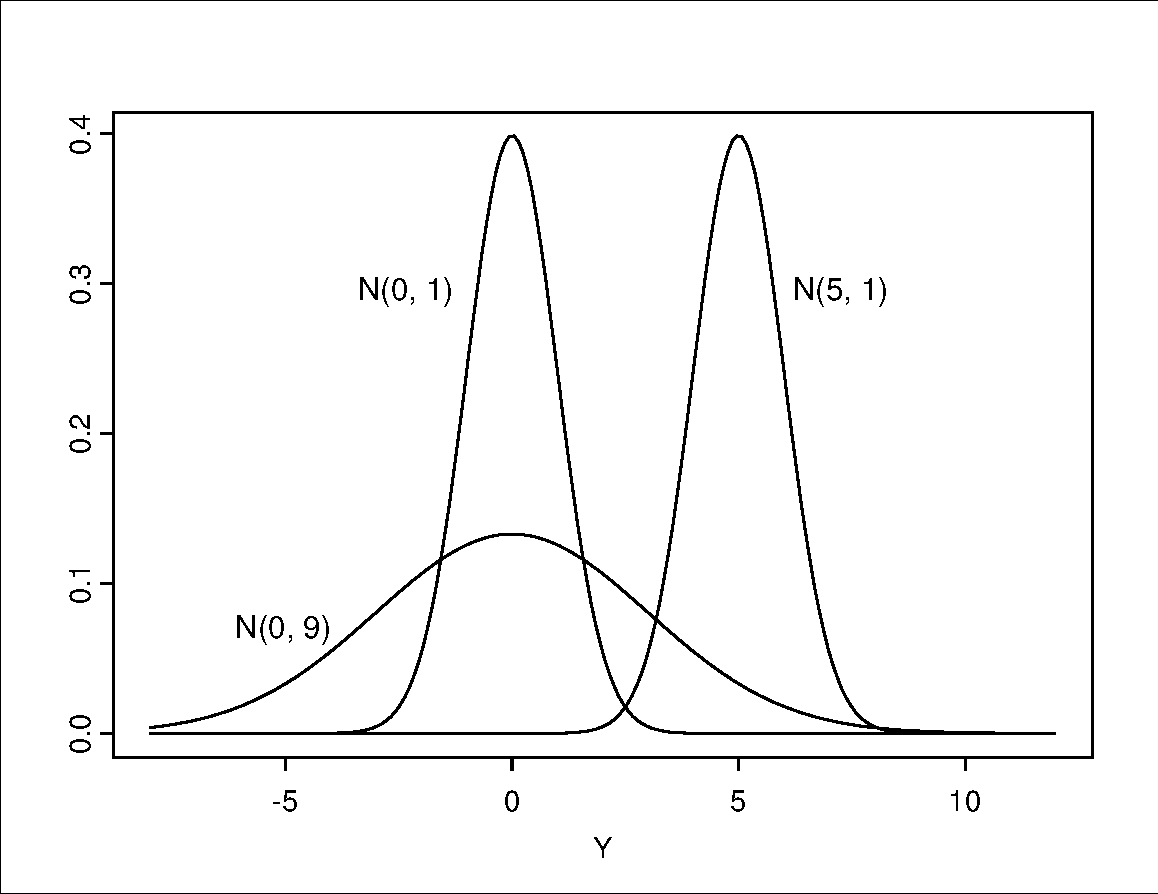
\includegraphics[height=8.5cm]{threenorms}
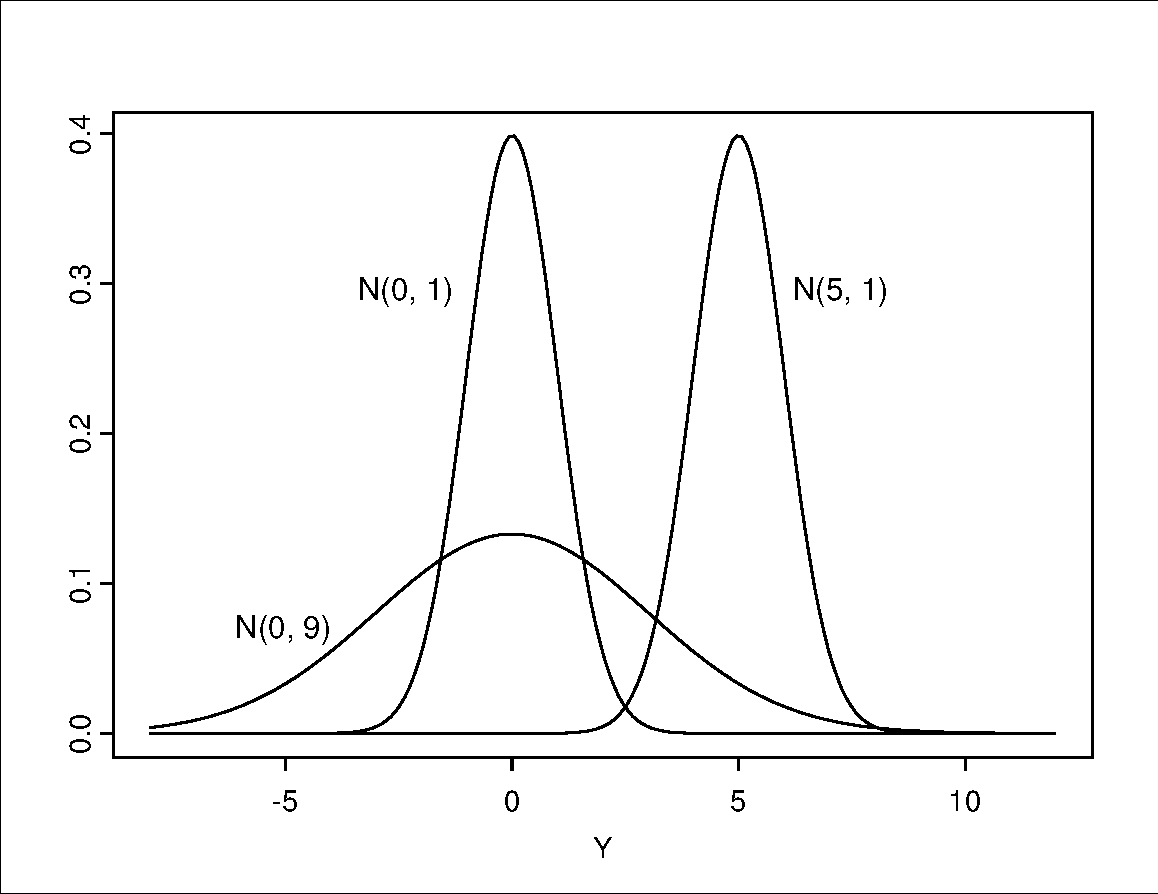
\includegraphics[width=11cm]{threenorms}
\end{center}
\vspace*{-2ex}
\end{figure}

The variance $\sigma^{2}$ determines how widely spread the curve is. In
Figure \ref{f_3norms}, the curves for $N(0, 1)$ and $N(5, 1)$ have the
same variance $\sigma^{2}=1$, so they have the same shape in
terms of their spread. The curve for $N(0, 9)$, on the other hand, is
more spread out, because it has a higher variance of $\sigma^{2}=9$. As
before, it is often more convenient to describe variability in terms of
the standard deviation $\sigma$, which is the square root of the
variance. Thus we may also say that the $N(0, 9)$ distribution has the
standard deviation $\sigma=\sqrt{9}=3$ (for $\sigma^{2}=1$ the two
numbers are the same, since $\sqrt{1}=1$).

In the histogram in Figure \ref{f_bp1}, the heights of the bars
correspond to the proportions of different ranges of blood
pressure among the 4489 people in the data set. Another way of stating
this is that if we were to sample a person from this group at random,
the heights of the
bars indicate the \textbf{probabilities} that the selected person's
blood pressure would be in a particular range. Some values are clearly
more likely than others. For example, for blood
pressures in the range 50--51.5, the probability is about 0.0025,
corresponding to a low bar, while for the range 74--75.5 it is about
0.0365, corresponding to a much higher bar.

The interpretation is the same for the curve of a continuous probability
distribution. Its height also indicates the probability of
different values in random sampling from a population
with that distribution. More precisely, the \emph{areas} under the curve
give such probabilities for ranges of values. Probabilities of all the
possible values must add up to one, so the area under the whole
curve is one --- i.e.\ a randomly sampled unit must have \emph{some}
value of the variable in question. More generally, the area under the
curve for a range of values gives the probability that the value of a
randomly sampled observation is in that range. These are the same
principles that we have already used to derive $P$-values for tests in
Sections \ref{ss_tables_chi2test_Pval} and
\ref{ss_probs_test1sample_samplingd}.

\begin{figure}[t]
\caption{Illustration of probabilities for the normal distribution.
The probability of an observation being within one standard deviation of
the mean (the grey area) is 0.68, and the probability of it being within
1.96 standard deviations of the mean (grey and shaded areas together) is
0.95.}
\label{f_norm1}
\begin{center}
%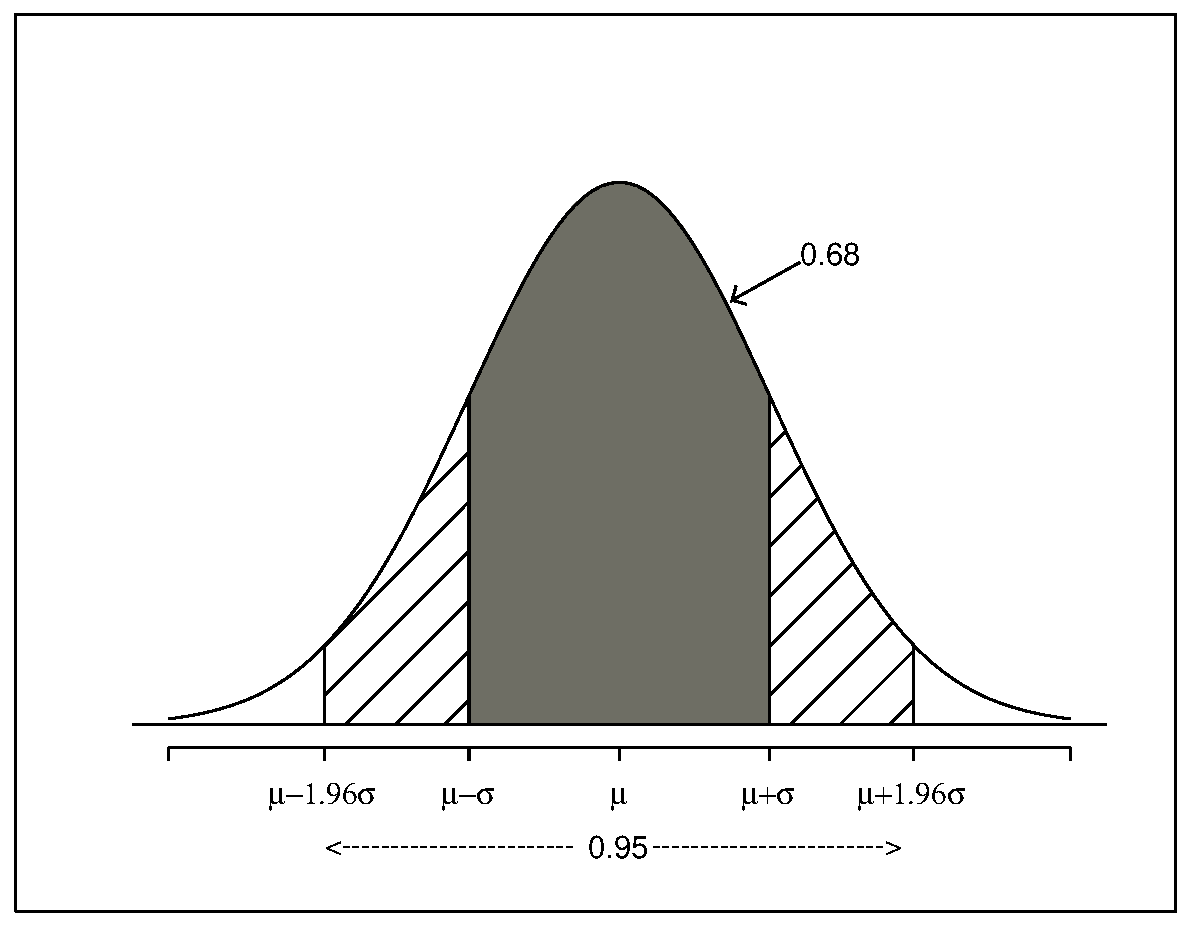
\includegraphics[height=8.5cm]{norm1}
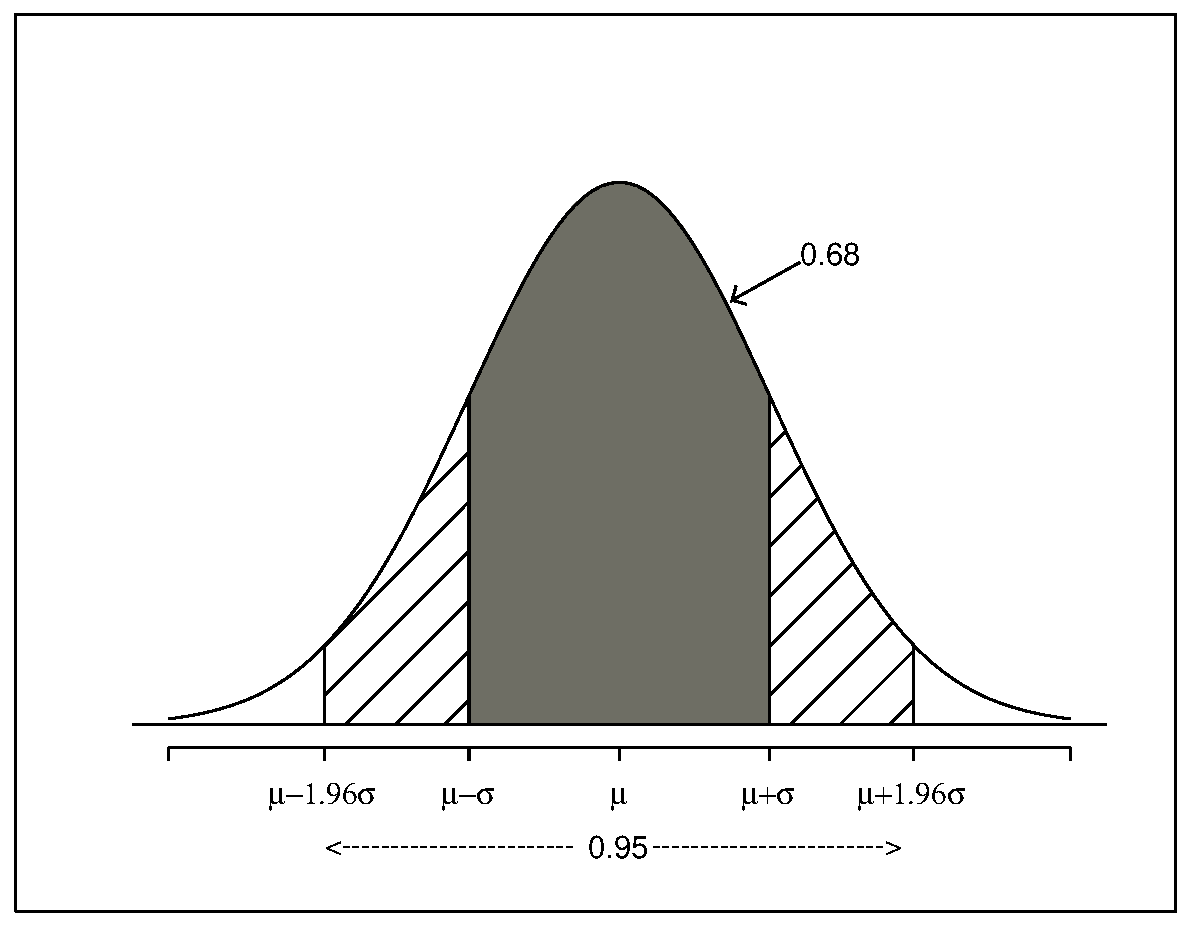
\includegraphics[width=12cm]{norm1}
\end{center}
\vspace*{-2ex}
\end{figure}

Figure \ref{f_norm1} illustrates this further with some results which hold for
any normal distribution, whatever its mean and variance. The grey area
in the figure corresponds to values from $\mu-\sigma$ to $\mu+\sigma$,
i.e.\ those values which are no further than one standard deviation from
the mean. The area of the grey region is 0.68, so the probability
that a randomly sampled value from a normal distribution is within one
standard deviation of the mean is 0.68. The two shaded regions either
side of the grey area extend the area to 1.96 standard deviations below
and above the mean. The probability of this region (the grey and shaded
areas together) is 0.95. Rounding the 1.96 to 2, we can thus say that
approximately 95\% of observations drawn from a normal distribution tend
to be within two standard deviations of the mean. This leaves the
remaining 5\% in the two tails of the distribution,
further than 1.96 standard deviations from the mean (the two white areas
in Figure \ref{f_norm1}). Because the normal distribution is symmetric,
these two areas are of equal size and each thus has the probability
0.025 (i.e.\ 0.05/2).

Such calculations can also be used to determine probabilities in particular
examples. Returning to the blood pressure data,
we might for example
be interested in
\vspace*{-2ex}
\begin{itemize}
\item
the proportion of people in some population whose diastolic blood
pressure is
higher than 90 (one possible cut-off point for high blood pressure or
hypertension)
\item
the proportion of people with diastolic blood pressure below 60
(possibly indicating unusually low blood pressure or hypotension)
\item
the proportion of people in the normal pressure range of 60--90
\end{itemize}
Such figures might be of interest for example for predicting health
service needs for treating hypertension. Suppose that we were reasonably
confident (perhaps from surveys like the one described above) that the
distribution of diastolic blood pressure in the population of interest
was approximately normally distributed with mean 74.2 and variance
127.87 (and thus standard deviation 11.3). The probabilities of interest
are then the areas of the regions shown in Figure \ref{f_normbp}.


The remaining question is how to calculate such probabilities. The
short answer is ``with a computer''. However, to explain
an approach which is required for this in some computer packages and also
to provide an alternative method which does not require a computer, we
need to introduce one more new quantity. This is the \textbf{Z score},
which is defined as
\begin{equation}
Z = \frac{Y-\mu}{\sigma}
\label{Zscore}
\end{equation}
where $Y$ can be any value of the variable of interest. For example, in
the blood pressure example the $Z$ scores corresponding to values 60 and
90 are $Z=(60-74.2)/11.3=-1.26$ and $Z=(90-74.2)/11.3=1.40$
respectively. The $Z$ score can be interpreted as the distance of the
value $Y$ from the mean $\mu$, measured in standard deviations $\sigma$.
Thus the blood pressure 60, with a $Z$ score of $-1.26$, is 1.26 standard
deviations \emph{below} (hence the negative sign) the mean, while 90
(with $Z$ score 1.40) is 1.40 standard deviations \emph{above} the mean.

\begin{figure}[t]
\caption{
Illustration of probabilities for a normal distribution in
the blood pressure example, where $\mu=74.2$ and $\sigma=11.3$. The
plot shows probabilities for the ranges of values at most 60
(``Low''), between 60 and 90 ("Mid'') and over 90 (``High'').
}
\label{f_normbp}
\begin{center}
%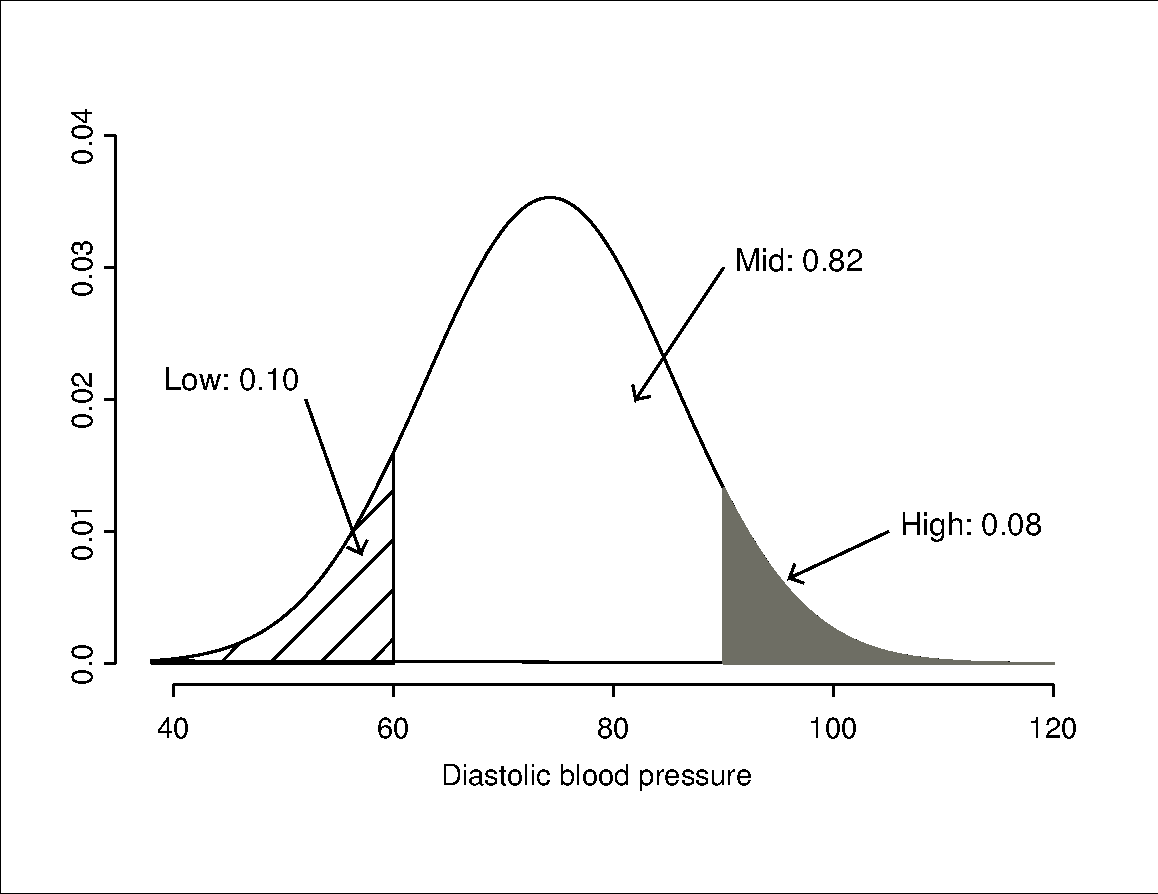
\includegraphics[height=8.5cm]{normbp}
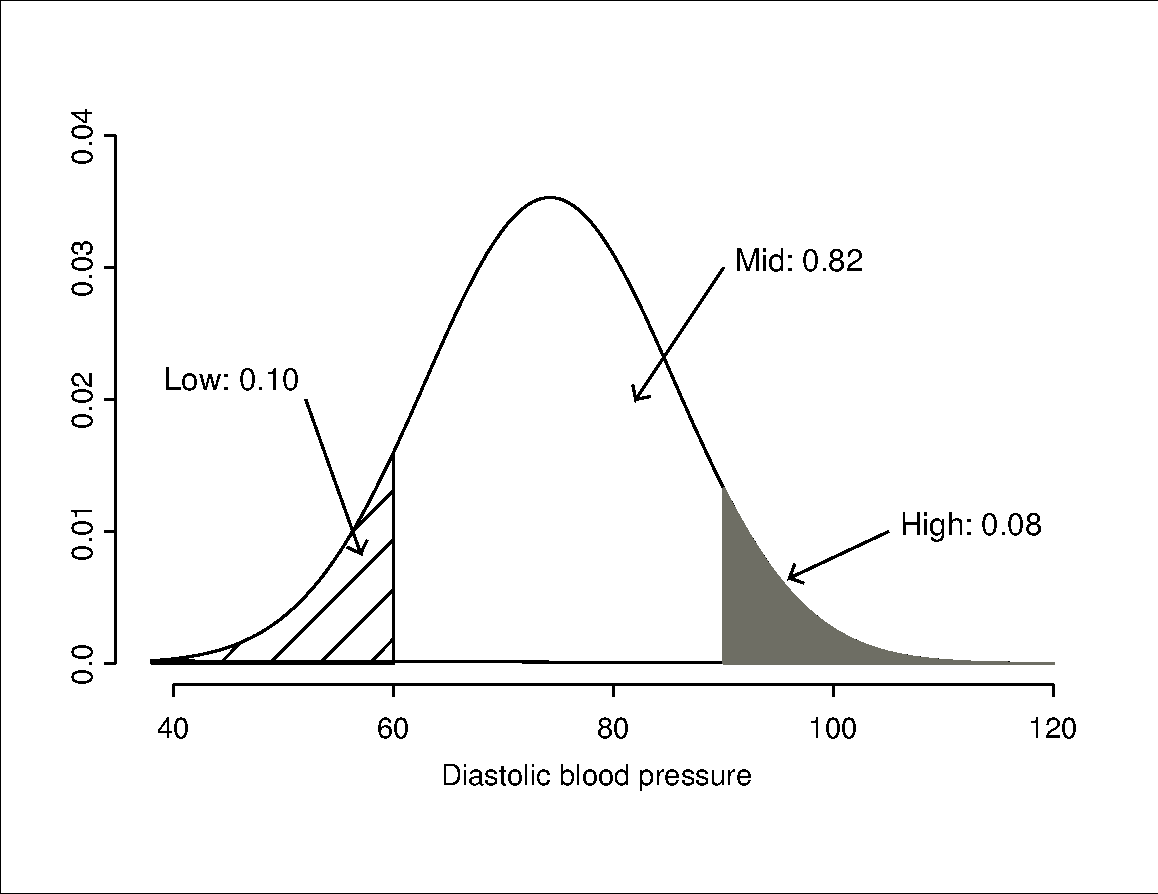
\includegraphics[width=12cm]{normbp}
\end{center}
\vspace*{-2ex}
\end{figure}

\begin{table}
\caption{Extract from the table of right-hand tail probabilities for
normal $Z$ scores. Here ``Tail Prob.'' is the probability that a
value from the standard normal distribution is at least the value
in the column labelled ``$z$''. The full table is shown on p.\
\pageref{s_disttables_Z}.}
\label{t_normtab}
\begin{center}
{\footnotesize
\begin{tabular}{|r|r|}\hline
\rule[1ex]{0mm}{2ex}$z$ & Tail Prob.\ \\
\hline
$\vdots$ & $\vdots$\\
1.24 & 0.1075 \\
1.25 & 0.1056 \\
1.26 & 0.1038 \\
1.27 & 0.1020 \\
$\vdots$ & $\vdots$ \\
1.38 & 0.0838\\
1.39 & 0.0823\\
1.40 & 0.0808\\
1.41 & 0.0793\\
$\vdots$ & $\vdots$ \\
\hline
\end{tabular}
}
\end{center}
\end{table}

The probability distribution of the $Z$ scores is a normal distribution
with mean 0 and variance 1, i.e.\ $Z\sim N(0,1)$. This is known as the
\textbf{standard normal distribution}. The usefulness of $Z$ scores lies
in the fact that by transforming the original variable $Y$ from the
$N(\mu, \sigma^{2}$) distribution into the standard normal distribution
they remove the specific values of $\mu$ and $\sigma$ from the
calculation. With this trick, probabilities for any normal distribution
can be calculated using a single table for $Z$ scores.
Such a table is given on page
\pageref{s_disttables_Z} in the Appendix, and an extract from it is
shown in Table
\ref{t_normtab} (note that it is not
always presented exactly like this, as different books may use slightly
different format or notation). The first column lists values of the $Z$
score (a full table would typically give
all values from 0.00 to about 3.50). The second column, labelled
``Tail Prob.'', gives the probability that a $Z$ score for a normal
distribution is \emph{larger than} the value given by $z$, i.e.\ the area of
the region to the right of $z$.

Consider first the probability that blood pressure is greater than 90,
i.e.\ the area labelled ``High'' in Figure \ref{f_normbp}. We have seen
that 90 corresponds to a $Z$ score of 1.40, so the probability of
high blood pressure is the same as the probability that the normal $Z$
score is greater than 1.40. The row for $z=1.40$ in the table tells us
that this probability is 0.0808, or 0.08 when rounded to two decimal
places as in Figure \ref{f_normbp}.

The second quantity of interest was the probability of a blood pressure
at most 60, i.e.\ the area of the ``Low'' region in Figure
\ref{f_normbp}. The corresponding $Z$ score is $-1.26$. The table,
however, shows only positive values of $z$. This is because we
can use the symmetry of the normal distribution to reduce all such
questions to ones about positive values of $z$. Because the
distribution is symmetric, the probability that a $Z$ score is \emph{at
most} $-1.26$ (the area of the left-hand tail to the left of $-1.26$)
is the same as the probability that it is \emph{at least} 1.26 (the area
of the right-hand tail to the right of 1.26).
This is the kind of quantity we calculated above\footnote{Note that there we were looking for the
probability of a Z score being ``bigger than'' rather than ``at least''
a certain value; for a continuous probability distribution this makes no
difference, and both probabilities are the same.}. The required
probability is thus equal to the right-hand tail probability for 1.26, which
the table shows to be 0.1038
(rounded to 0.10 in Figure
\ref{f_normbp}).

Finally, the probability of the ``Mid'' range of blood pressure is the
remaining probability not in the two other regions. Because the whole
area under the curve (the total probability) is 1, the required
probability is obtained by subtraction as $1-(0.0808+0.1038)=0.8154$. In this example these values
obtained from the normal approximation of the population distribution
are very accurate. The exact proportions of the 4489 respondents who had
diastolic blood pressure at most 60 or greater than 90 were 0.0996 and
0.0793 respectively, so rounded to two decimal places they were the same
as the 0.10 and 0.08 obtained from the normal approximation.

\label{p_cdfnorm}
These days we can use statistical computer programs
to calculate such
probabilities directly for a normal distribution with any mean and
standard deviation. For example, SPSS has a function called
\texttt{CDF.NORMAL(}\emph{quant,mean,stddev}\texttt{)} for this purpose.
It calculates the probability that the value from a normal distribution
with mean \emph{mean} and standard deviation \emph{stddev} is \textbf{at most}
\emph{quant}.

In practice we do not usually know the population mean and variance, so
their sample estimates will be used in such calculations. For example,
for the sample in Table \ref{t_bp_example} we had $\bar{Y}=72.6$ and
$s=12.7$. Using these values in a similar calculation as above gives the
estimated proportion of people in the population with diastolic blood
pressures over 90 as 8.5\%. Even with a sample of only 50 observations,
the estimate is reasonably close to the true population proportion of
about 8.1\%.

\section{The normal distribution as a sampling distribution}
\label{s_contd_clt}

We have already encountered the normal distribution in Section
\ref{ss_probs_test1sample_samplingd}, in the role of the \emph{sampling
distribution} of a test statistic rather than as a model for the population
distribution of a variable. In fact, the most important use of the
normal distribution is as a sampling distribution, because in this role
it often cannot be replaced by any other simple distributions. The
reasons for this claim are explained in this section. We begin with the
case of the distribution of the sample mean in samples from a
normal population, before extending it with a result
which provides the justification for the
standard normal sampling distributions used for inference on proportions
in Chapter \ref{c_probs}, and even for the $\chi^{2}$ sampling distribution
of the $\chi^{2}$ test in Chapter \ref{c_tables}.

Recall from Section \ref{ss_tables_chi2test_sdist} that the sampling
distribution of a statistic is its distribution across all possible
random samples of a given size from a population. The statistic we focus
on here is the sample mean $\bar{Y}$. If we assume that the population
distribution is exactly normal, we have the following result:
\begin{itemize}
\item
If the population distribution of a variable $Y$ is normal with mean
$\mu$ and variance $\sigma^{2}$, the sampling distribution of the sample
mean $\bar{Y}$ for a random sample of size $n$ is also a normal
distribution, with mean $\mu$ and variance $\sigma^{2}/n$.
\end{itemize}
The mean and variance of this sampling distribution
are worth discussing separately:
\begin{itemize}
\item
The mean of the sampling distribution of $\bar{Y}$ is equal to the
population mean $\mu$ of $Y$.
This means that while $\bar{Y}$ from a single sample may be below or above the true
$\mu$, in repeated samples it would on average estimate the correct
parameter.
In statistical language, $\bar{Y}$
is then an \emph{unbiased estimate} of $\mu$.
More generally,
most possible samples would give values of $\bar{Y}$ not very far from
$\mu$, where the scale for ``far'' is provided by the standard deviation
discussed below.
\item
The variance of the sampling distribution of $\bar{Y}$ is $\sigma^{2}/n$
or, equivalently, its standard deviation is $\sigma/\sqrt{n}$. This
standard deviation is also known as the \textbf{standard error of the
mean}, and is often denoted by something like
$\sigma_{\bar{Y}}$. It describes the variability of the sampling
distribution. Its magnitude depends on $\sigma$, i.e.\ on the
variability of $Y$ in the population. More interestingly, it also
depends on the sample size $n$, which appears in the denominator in
$\sigma/\sqrt{n}$. This means that the standard error of the mean is
smaller for large samples than for small ones. This is illustrated in
Figure \ref{f_sampld2}. It shows the sampling distribution of $\bar{Y}$
for samples of sizes $n=50$ and $n=1000$ from a normal population with
$\mu=74.2$ and $\sigma=11.3$, i.e.\ the population mean and standard
deviation in the blood pressure example.
It can be seen that while both sampling
distributions are centered around the true mean $\mu=74.2$, the
distribution for the smaller sample is more spread out than that for the
larger sample: more precisely, the standard error of the mean is
$\sigma/\sqrt{n}=11.3/\sqrt{50}=1.60$ when $n=50$ and
$11.3/\sqrt{1000}=0.36$
when $n=1000$. Recalling from Section
\ref{ss_contd_probdistrs_normal} that
approximately 95\% of the probability in a normal distribution is
within two standard deviations of the mean, this means that about 95\%
of samples of size 50 in this case would give a value of $\bar{Y}$
between $\mu-2*1.60=74.2-3.2=71.0$ and $74.2+3.2=77.4$. For samples of size
$n=1000$, on the other hand, 95\% of samples would yield
$\bar{Y}$ in the much narrower range of $74.2-2*0.36=73.5$ to
$74.2+2*0.36=74.9$.
\end{itemize}

\begin{figure}
\caption{Illustration of the sampling distribution of the sample mean
for two sample sizes. In both cases the population distribution is
normal with $\mu=74.2$ and $\sigma=11.3$.
}
\label{f_sampld2}
\vspace*{-2ex}
\begin{center}
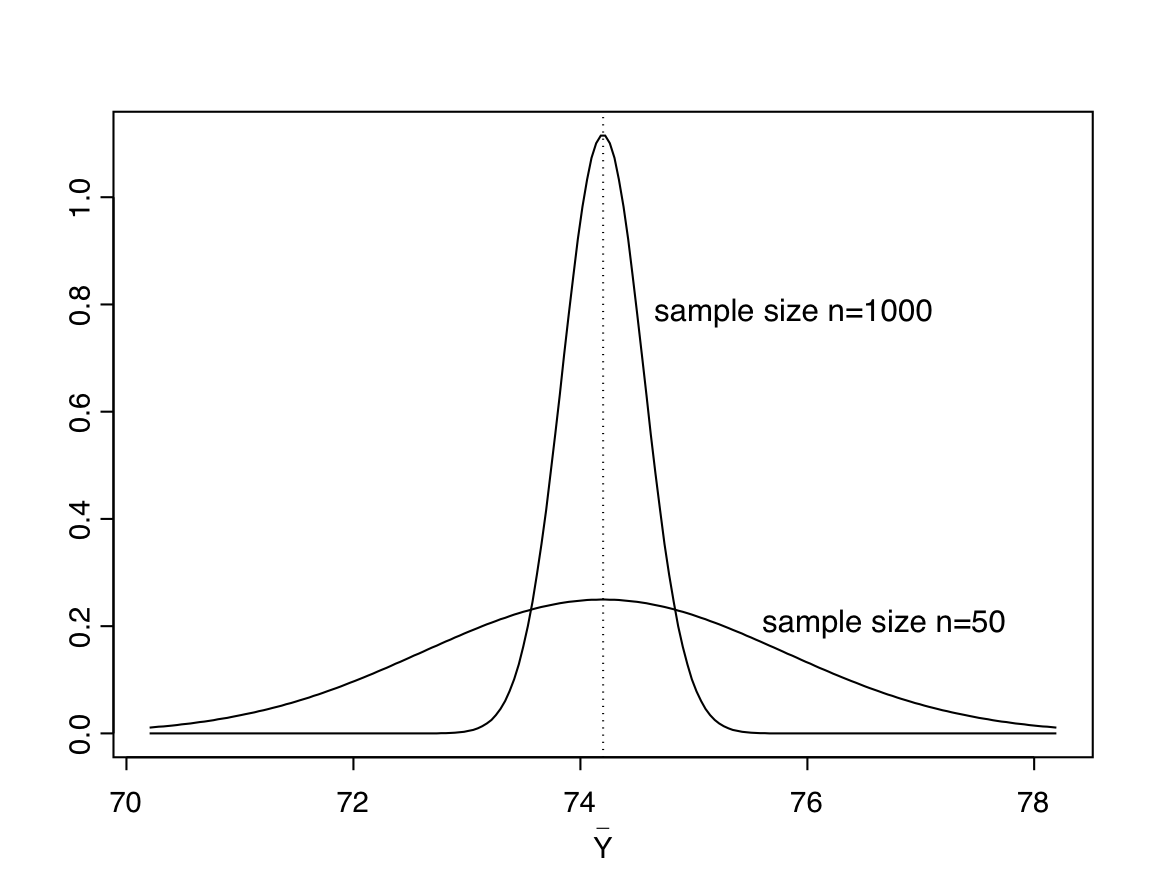
\includegraphics[width=12cm]{sampld2_bp}
\end{center}
\vspace*{-3ex}
\end{figure}

The connection between sample size and the variability of a sampling
distribution applies not only to the sample mean but to (almost) all
estimates of population parameters. In general, (i) the task of
statistical inference is to use information in a sample to draw
conclusions about population parameters; (ii)
the expected magnitude of the sampling error, i.e.\
the remaining uncertainty about population parameters
resulting from having information only on a sample, is characterised by
the variability of the sampling distributions of estimates of the
parameters; and (iii) other things being equal, the variability of a
sampling distribution decreases when the sample size increases. Thus
data really are the currency of statistics and more data
are better than less data. In practice data collection of course costs
time and money, so we cannot always obtain samples which are as large as
we might otherwise want. Apart from resource constraints, the choice of
sample size depends also on such things as the aims of the
analysis, the level of precision required, and guesses about the
variability of variables in the population. Statistical
considerations of the trade-offs between them in order to make
decisions about sample sizes are known as
\emph{power} calculations. They will be discussed very briefly later, in
Section \ref{ss_means_tests3_power}.

In Figure \ref{f_sampld} we use a computer simulation rather than a
mathematical theorem to examine the sampling distribution of a sample
mean. Here 100,000 simple random samples of
size $n=50$ were drawn from the $N=4489$ values of blood
pressure that we are treating as the finite population in this
illustration. The sample mean $\bar{Y}$ of blood pressure was calculated
for each of these samples, and the histogram of these 100,000 values of
$\bar{Y}$ is shown in Figure \ref{f_sampld}. Also shown is the curve of
the normal distribution with the mean $\mu$ and standard deviation
$\sigma/\sqrt{50}$ determined by the theoretical result given above.

\begin{figure}[t]
\caption{Example of the sampling distribution of the sample mean. The
plot shows a histogram of the values of the sample mean in 100,000 samples
of size $n=50$ drawn from the 4489 values of diastolic blood pressure
shown in Figure \ref{f_bp1}, for which the mean is $\mu=74.2$ and
standard deviation is $\sigma=11.3$.
Superimposed on the histogram
is the curve of the approximate sampling
distribution, which is normal with mean $\mu$ and standard
deviation $\sigma/\sqrt{n}$.
}
\label{f_sampld}
\begin{center}
\vspace*{-2ex}
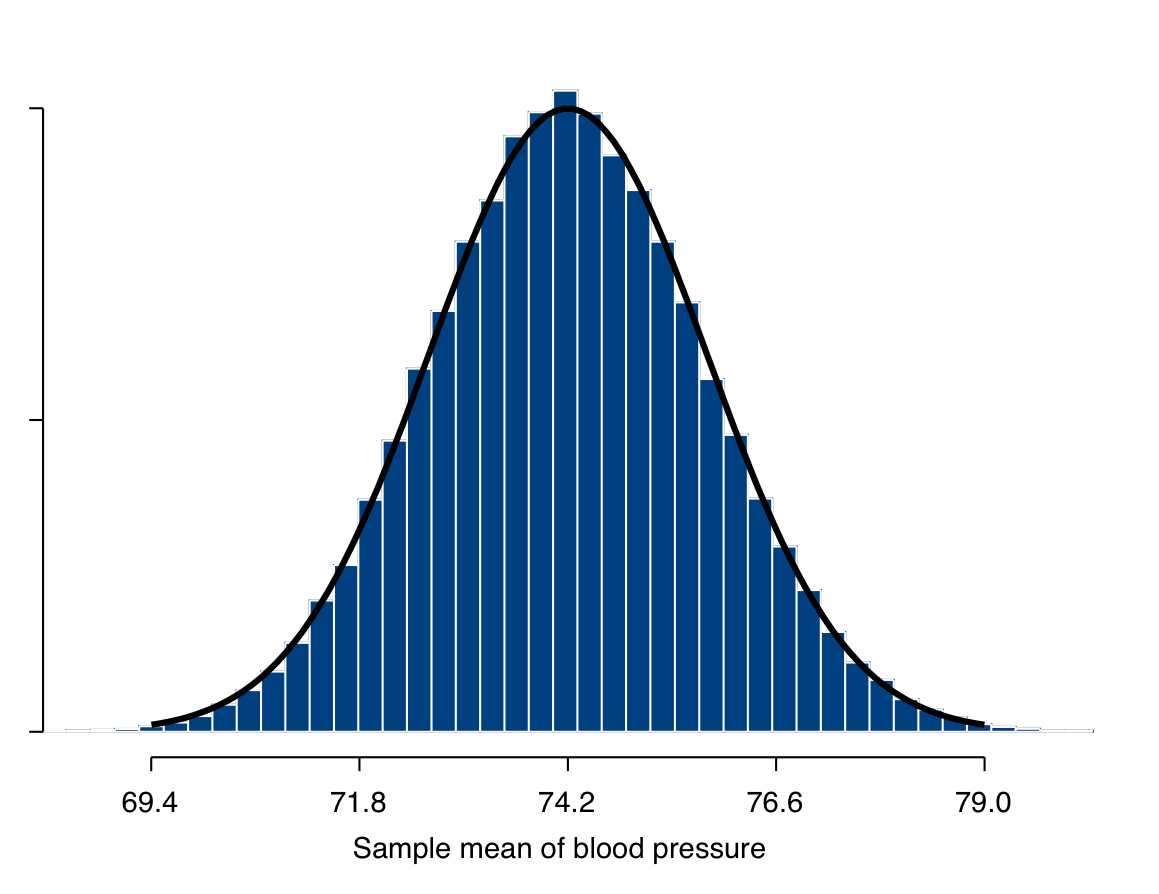
\includegraphics[width=12cm]{sampld1_bp}
\end{center}
\vspace*{-2ex}
\end{figure}

The match between the curve and the histogram in Figure \ref{f_sampld}
is clearly very close. This is actually a nontrivial finding which
illustrates a result which is of crucial importance for statistical
inference. Recall that the normal curve shown in Figure \ref{f_sampld}
is derived from the mathematical result stated above, which assumed that
the population distribution of $Y$ is \emph{exactly} normal. The
histogram in Figure \ref{f_sampld}, on the other hand, is based on
repeated samples from the actual population distribution of blood
pressure, which, while quite close to a normal distribution as shown in
Figure \ref{f_bp2}, is certainly not exactly normal. Despite this, it is
clear that the normal curve describes the histogram essentially exactly.

If this was not true, that is if the sampling distribution
that applies for the normal distribution was inadequate when the the true
population distribution was even slightly different from normal, the
result would be of little practical use. No population
distribution is ever exactly normal, and many are very far from
normality. Fortunately, however, it turns out that quite the opposite is
true, and that the sampling distribution of the mean is approximately
the same for nearly \emph{all} population distributions. This is the
conclusion from the \textbf{Central Limit Theorem} (CLT), one of the
most remarkable results in all of mathematics. Establishing the CLT with
increasing levels of generality has been the work of many mathematicians
over several centuries, as different versions of it have been proved by,
among others, de Moivre, Laplace, Cauchy, Chebyshev, Markov, Liapounov,
Lindeberg, Feller, L\'{e}vy, Hoeffding, Robbins, and Rebolledo between
about 1730 and 1980. One version of the CLT can be stated as

\textbf{The (Lindeberg-Feller) Central Limit Theorem}: For each
$n=1,2,\dots$, let $Y_{nj}$, for $j=1,2,\dots,n$, be independent random
variables with $\text{E}(Y_{nj})=0$ and $\text{var}(Y_{nj})=\sigma^{2}_{nj}$. Let
$Z_{n}=\sum_{j=1}^{n} Y_{nj}$, and let
$B^{2}_{n}=\text{var}(Z_{n})=\sum_{j=1}^{n} \sigma^{2}_{nj}$. Suppose also
that the following condition holds: for every $\epsilon>0$,
\begin{equation}
\frac{1}{B_{n}^{2}}\,
\sum_{j=1}^{n} \, \text{E}\{ Y_{nj}^{2} I(|Y_{nj}|\ge \epsilon B_{n})\}
\rightarrow 0 \; \text{  as  } \; n\rightarrow \infty.
\label{lindeberg}
\end{equation}
Then $Z_{n}/B_{n} \stackrel{\mathcal{L}}{\longrightarrow} N(0,1)$.

No, that will not come up in the examination. The theorem is given here
just as a glimpse of how this topic would be introduced in
a very different kind of text book\footnote{Ferguson, T.\ S.\ (1996). \emph{A Course in Large Sample
Theory}, Chapman \& Hall, London.}, and because it pleases the author of this
coursepack to note that Jarl Lindeberg was Finnish. For our purposes, it is
better to state the same result in English:
\begin{itemize}
\item
If $Y_{1}, Y_{2}, \dots, Y_{n}$ are a random sample of observations from
(almost\footnote{The CLT does not hold in some rather weird cases which
need not concern us here. Condition (\ref{lindeberg}) is a mathematical
expression for ``not weird''.}) any distribution with a population mean
$\mu$ and variance $\sigma^{2}$, and if $n$ is reasonably large, the
sampling distribution of their sample mean $\bar{Y}$ is approximately a
normal distribution with mean $\mu$ and variance $\sigma^{2}/n$.
\end{itemize}
Thus the sampling distribution of the mean from practically any
population distribution is approximately the same as when the population
distribution is normal, as long as the sample size is ``reasonably
large''. The larger the sample size is, the closer the sampling
distribution is to the normal distribution, and it becomes exactly
normal when the sample size is infinitely large (i.e.\
``asymptotically''). What is large enough depends particularly on the
nature of the population distribution. For continuous variables, the CLT
approximation is typically adequate even for sample sizes as small as
$n=30$, so we can make use of the approximate normal sampling
distribution when $n$ is 30 or larger. This is, of course, simply a
pragmatic rule of thumb which does not mean that the normal
approximation is completely appropriate for $n=30$ but entirely
inappropriate for $n=29$; rather, the approximation becomes better and
better as the sample size increases, while below about 30 the chance of
incorrect conclusions from using it becomes large enough for us not to
usually want to take that risk.

We have seen in Figure \ref{f_sampld2} that in the blood pressure
example the sampling distribution given by the Central Limit Theorem is
essentially exact for samples of size $n=50$. In this case this is
hardly surprising, as the population distribution itself is already
quite close to a normal distribution. The theorem is not, however,
limited to such easy cases but works quite generally. To demonstrate
this with a more severe test, let us consider a population distribution
that is as far as possible from normal. This is the binomial
distribution of a binary variable that was introduced in Section
\ref{s_probs_distribution}. If the probability parameter of this
distribution is $\pi$, its mean and variance are $\mu=\pi$ and
$\sigma^{2}=\pi(1-\pi)$, and the sample mean $\bar{Y}$ of observations from
the distribution is the sample
proportion $\hat{\pi}$ (see
equation
\ref{pihat_as_ybar} on page
\pageref{pihat_as_ybar}).
The CLT then tells us that
\begin{itemize}
\item
When $n$ is large enough, the sampling distribution of
the sample proportion
$\hat{\pi}$ of a dichotomous variable $Y$ with population
proportion $\pi$ is approximately a normal distribution with mean $\pi$
and  variance $\pi(1-\pi)/n$.
\end{itemize}
This powerful result is illustrated in Figure \ref{f_cltbin}. It is
similar to Figure \ref{f_sampld}
in that it shows sampling distributions
obtained from a computer simulation, together with the normal curve
suggested by the CLT. For each plot, 5000 samples of size $n$ were
simulated from a population where $\pi$ was 0.2. The sample
proportion $\hat{\pi}$ was then calculated for each simulated sample,
and the histogram of these 5000 values drawn. Four different sample
sizes were used: $n=10$, 30, 100, and 1000. It can be seen that
the normal distribution is not a very good approximation of
the sampling distribution of $\hat{\pi}$ when $n$ is as small as 10 or
even 30. For the larger values of 100 and 1000, however, the normal
approximation is already quite good, as expected from the CLT.

\begin{figure}[t]
\caption{Illustration of the Central Limit Theorem for the sample
proportion of a dichotomous variable. Each plot shows the histogram of
the sample proportions $\hat{\pi}$ calculated for 5000 samples simulated
from a population distribution with proportion $\pi=0.2$, together with
the normal curve with mean $\pi$ and variance $\pi(1-\pi)/n$. The
samples sizes $n$ are 10, 30, 100 and 1000.}
\label{f_cltbin}
\begin{center}
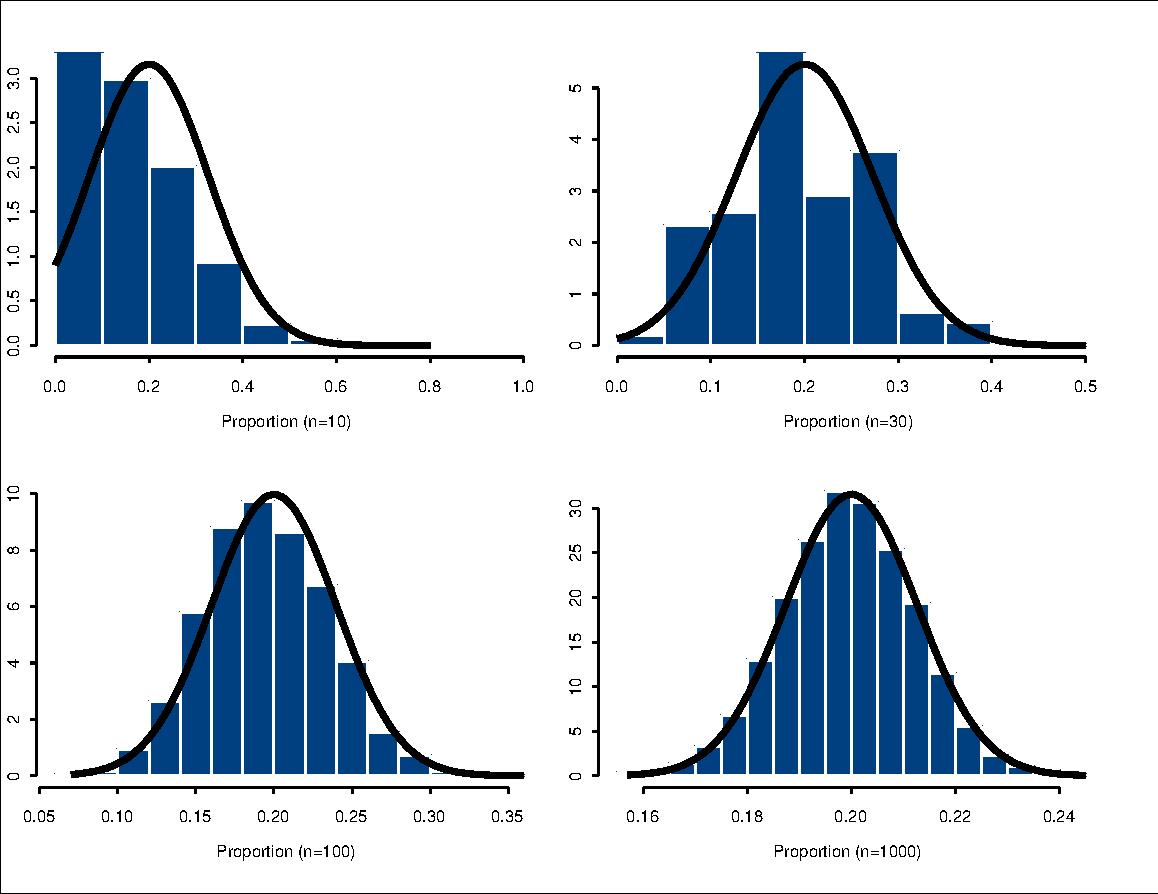
\includegraphics[width=140mm]{sampld_p}
\end{center}
\vspace*{-2ex}
\end{figure}

The variability of the sampling distribution will again depend on $n$.
In Figure \ref{f_cltbin}, the observed range of values of
$\hat{\pi}$ decreases
substantially as $n$ increases. When $n=10$, values of between about 0
and 0.4 are quite common, whereas with $n=1000$, essentially all of the
samples give $\hat{\pi}$ between about 0.16 and 0.24, and a large
majority are between 0.18 and 0.22. Thus increasing the sample size will
again increase the precision with which we can estimate $\pi$, and decrease
the uncertainty in inference about its true value.

The Central Limit Theorem is, with some additional results, the
justification for the standard normal sampling distribution used for
tests and confidence intervals for proportions in Chapter \ref{c_probs}.
The conditions for sample sizes mentioned there (pages
\pageref{p_thumbp} and \pageref{p2pthumb}) again derive from conditions
for the CLT to be adequate. The same is also ultimately true for the
$\chi^{2}$ distribution and conditions for the $\chi^{2}$ test in Chapter
\ref{c_tables}. Results like these, and many others, explain the central
importance of the CLT in statistical methodology.

